% Chapter 4
\chapter{Face Detection} % Main chapter title

\label{Chapter4} % For referencing the chapter elsewhere, use \ref{Chapter1}

\lhead{Chapter 4. \emph{Face Detection}} % This is for the header on each page - perhaps a shortened title

A face detector has to tell whether an image of arbitrary size contains a human face and if so, where
it is. One natural framework for considering this problem is that of binary classification, in which
a classifier is constructed to minimize the misclassification risk. Since no objective distribution can
describe the actual prior probability for a given image to have a face, the algorithm must minimize
both the false negative and false positive rates in order to achieve an acceptable performance.
This task requires an accurate numerical description of what sets human faces apart from other
objects. It turns out that these characteristics can be extracted with a remarkable committee learning
algorithm called Adaboost, which relies on a committee of weak classifiers to form a strong
one through a voting mechanism. An operational algorithm must also work with a reasonable computational 
budget. Techniques such as integral image and attentional cascade make the Viola-Jones algorithm \cite{Viola2004RRF966432}
highly efficient: fed with a real time image sequence generated from a standard webcam, it performs well on a
standard PC.\cite{ipol.2014.104}

%----------------------------------------------------------------------------------------
\section{Robust Real-time Object Detection}
The Viola-Jones algorithm  \cite{Viola2004RRF966432}, the first ever real-time face detection system. 
There are three contributions of Viola-Jones algorithm to enable a fast and accurate detection:
the \textbf{integral image} for feature computation, \textbf{Adaboost} for feature selection and an 
\textbf{attentional cascade} for efficient computational resource allocation. 
Since the Viola-Jones algorithm typically gives multiple detections, 
a post-processing step is also proposed to reduce detection redundancy using a robustness argument.\cite{ipol.2014.104}


\begin{compactitem}
\item {Features}
The Viola-Jones object detection procedure classifies images based on the value of simple features.
There are many motivations for using features rather than the pixels directly. The feature-based system 
operates much faster than a pixel-based system.
The simple features used are Haar basis functions. There are three kinds of features used. 
The value of a two-rectangle feature is the difference between the sum of the pixels within
two rectangular regions. The regions have the same size and shape and are horizontally
or vertically adjacent (see \autoref{fig:chap4-Haar}). A three-rectangle feature computes the sum within
two outside rectangles subtracted from the sum in a center rectangle. Finally a fourrectangle
feature computes the difference between diagonal pairs of rectangles.
Given that the base resolution of the detector is 24x24, the exhaustive set of rectangle
features is quite large, 45,396.

\begin{figure}[h]
  \centering
	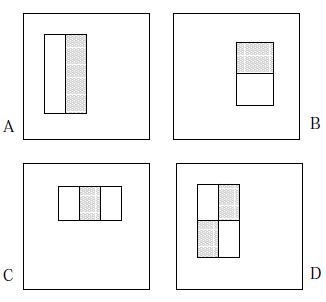
\includegraphics[width=0.7\textwidth, keepaspectratio=true]{chap4-Haar.png}
  \caption{Example rectangle features shown relative to the enclosing detection window.
The sum of the pixels which lie within the white rectangles are subtracted from the
sum of pixels in the grey rectangles. Two-rectangle features are shown in (A) and (B).
Figure (C) shows a three-rectangle feature, and (D) a four-rectangle feature.}
  \label{fig:chap4-Haar}
\end{figure}

\item {Integral Image}
Rectangle features can be computed very rapidly using an intermediate representation
for the image which we call the integral image. The integral image at location x, y
contains the sum of the pixels above and to the left of x, y, inclusive:
$ii(x; y) = X x0x;y0yi(x0; y0);$
where $ii(x, y)$ is the integral image and $i(x, y)$ is the original image (see \autoref{fig:chap4-Integral}).
Using the following pair of recurrences:
%s(x; y) = s(x; y 􀀀 1) + i(x; y) (1)
%ii(x; y) = ii(x 􀀀 1; y) + s(x; y) (2)
%(where s(x; y) is the cumulative row sum, s(x;􀀀1) = 0, and ii(􀀀1; y) = 0) the
integral image can be computed in one pass over the original image.
Using the integral image any rectangular sum can be computed in four array references
(see  \autoref{fig:chap4-Integral4}). Clearly the difference between two rectangular sums can be
computed in eight references. Since the two-rectangle features defined above involve
adjacent rectangular sums they can be computed in six array references, eight in the
case of the three-rectangle features, and nine for four-rectangle features.
One alternative motivation for the integral image comes from the “boxlets” work
of Simard, et al.
\begin{figure}[h]
  \centering
	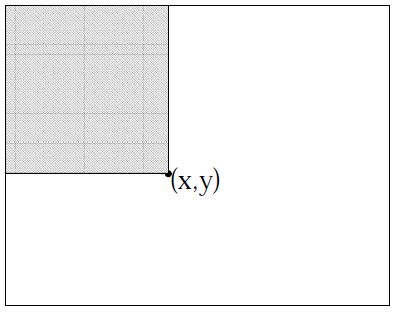
\includegraphics[width=0.7\textwidth, keepaspectratio=true]{chap4-Integral.png}
  \caption{The value of the integral image at point (x; y) is the sum of all the pixels
above and to the left.}
  \label{fig:chap4-Integral}
\end{figure}

\begin{figure}[h]
  \centering
	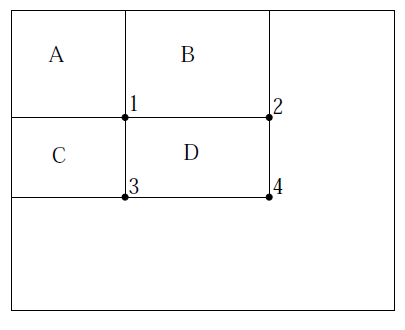
\includegraphics[width=0.7\textwidth, keepaspectratio=true]{chap4-Integral4.png}
  \caption{The sum of the pixels within rectangle D can be computed with four array
references. The value of the integral image at location 1 is the sum of the pixels in
rectangle A. The value at location 2 is A + B, at location 3 is A + C, and at location
4 is A + B + C + D. The sum within D can be computed as 4 + 1 - (2 + 3)}
  \label{fig:chap4-Integral4}
\end{figure}


\item {Feature Selection with Adaboost}
\item {The Attentional Cascade}
This section describes an algorithm for constructing a cascade of classifiers which
achieves increased detection performance while radically reducing computation time.
The key insight is that smaller, and therefore more efficient, boosted classifiers can be
constructed which reject many of the negative sub-windows while detecting almost all
positive instances. Simpler classifiers are used to reject the majority of sub-windows
before more complex classifiers are called upon to achieve low false positive rates.
Stages in the cascade are constructed by training classifiers using AdaBoost. Starting
with a two-feature strong classifier, an effective face filter can be obtained by adjusting
the strong classifier threshold to minimize false negatives. The initial AdaBoost
threshold, 
%1
%2 PT t=1 t, 
is designed to yield a low error rate on the training data. A lower
threshold yields higher detection rates and higher false positive rates. Based on performance
measured using a validation training set, the two-feature classifier can be
adjusted to detect 100% of the faces with a false positive rate of 40%. See Figure 5 for
a description of the two features used in this classifier.
The detection performance of the two-feature classifier is far from acceptable as an
object detection system. Nevertheless the classifier can significantly reduce the number
of sub-windows that need further processing with very few operations:
1. Evaluate the rectangle features (requires between 6 and 9 array references per
feature).
2. Compute the weak classifier for each feature (requires one threshold operation
per feature).
3. Combine the weak classifiers (requires one multiply per feature, an addition, and
finally a threshold).
A two feature classifier amounts to about 60 microprocessor instructions. It seems
hard to imagine that any simpler filter could achieve higher rejection rates. By comparison,
scanning a simple image template, or a single layer perceptron, would require at
least 20 times as many operations per sub-window.
The overall form of the detection process is that of a degenerate decision tree, what
we call a “cascade” [9] (see Figure 6). A positive result from the first classifier triggers
the evaluation of a second classifier which has also been adjusted to achieve very high
detection rates. A positive result from the second classifier triggers a third classifier,
and so on. A negative outcome at any point leads to the immediate rejection of the
sub-window.
The structure of the cascade reflects the fact that within any single image an overwhelming
majority of sub-windows are negative. As such, the cascade attempts to
reject as many negatives as possible at the earliest stage possible. While a positive
instance will trigger the evaluation of every classifier in the cascade, this is an exceedingly
rare event.
Much like a decision tree, subsequent classifiers are trained using those examples
which pass through all the previous stages. As a result, the second classifier faces a
more difficult task than the first. The examples which make it through the first stage are
“harder” than typical examples. The more difficult examples faced by deeper classifiers
push the entire reciever operating characteristic (ROC) curve downward. At a given
detection rate, deeper classifiers have correspondingly higher false positive rates.

\begin{figure}[h]
  \centering
	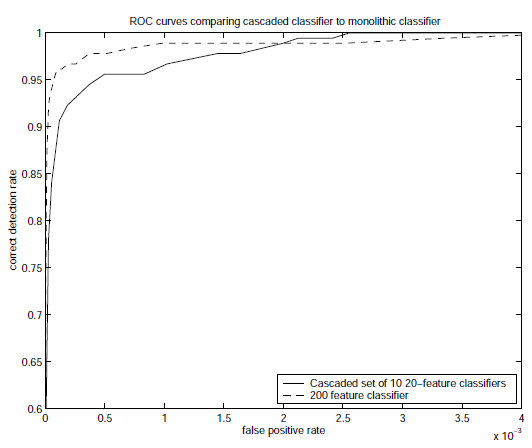
\includegraphics[width=0.7\textwidth, keepaspectratio=true]{chap4-ROC.png}
  \caption{Reciever operating characteristic (ROC) curve for the 200 feature classifier.}
  \label{fig:chap4-ROC}
\end{figure}

\begin{figure}[h]
  \centering
	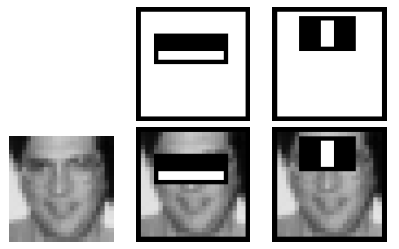
\includegraphics[width=0.7\textwidth, keepaspectratio=true]{chap4-Face.png}
  \caption{The first and second features selected by AdaBoost. The two features are
shown in the top row and then overlayed on a typical training face in the bottom row.
The first feature measures the difference in intensity between the region of the eyes and
a region across the upper cheeks. The feature capitalizes on the observation that the
eye region is often darker than the cheeks. The second feature compares the intensities
in the eye regions to the intensity across the bridge of the nose}
  \label{fig:chap4-Face}
\end{figure}


\begin{figure}[h]
  \centering
	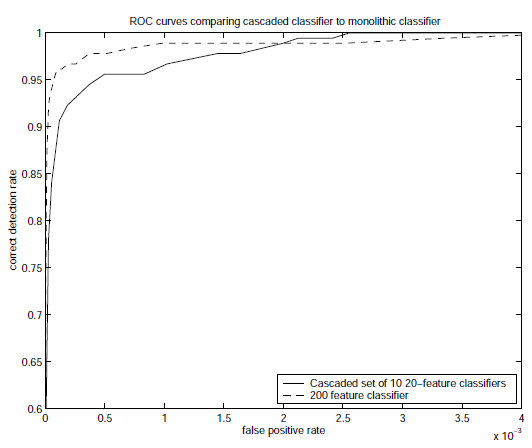
\includegraphics[width=0.7\textwidth, keepaspectratio=true]{chap4-Cascade.png}
  \caption{Schematic depiction of a the detection cascade. A series of classifiers are applied
to every sub-window. The initial classifier eliminates a large number of negative
examples with very little processing. Subsequent layers eliminate additional negatives
but require additional computation. After several stages of processing the number of
sub-windows have been reduced radically. Further processing can take any form such
as additional stages of the cascade (as in our detection system) or an alternative detection
system..}
  \label{fig:chap4-Cascade}
\end{figure}

\end{compactitem}

\section{PICO}
Object Detection with Pixel Intensity Comparisons Organized in Decision Trees
\cite{DBLPjournalscorrabs}

\section{NPD}

%----------------------------------------------------------------------------------------

